\documentclass{article}

\usepackage{graphicx} % For including graphics
\usepackage{amsmath} % For mathematical symbols and equations
\usepackage{fancyhdr}
\usepackage{hyperref} % For hyperlinks
\usepackage{listings} % For including code
\usepackage{xcolor}   % For colored text and backgrounds
\usepackage[utf8]{inputenc}
\usepackage[T1]{fontenc}
\usepackage[english,greek]{babel}
% Define colors for code listing
\definecolor{codegreen}{rgb}{0,0.6,0}
\definecolor{codegray}{rgb}{0.5,0.5,0.5}
\definecolor{codepurple}{rgb}{0.58,0,0.82}
\definecolor{backcolour}{rgb}{0.95,0.95,0.92}

% Code listing style
\lstdefinestyle{mystyle}{
    backgroundcolor=\color{backcolour},   
    commentstyle=\color{codegreen},
    keywordstyle=\color{magenta},
    numberstyle=\tiny\color{codegray},
    stringstyle=\color{codepurple},
    basicstyle=\ttfamily\footnotesize,
    breakatwhitespace=false,         
    breaklines=true,                 
    captionpos=b,                    
    keepspaces=true,                 
    numbers=left,                    
    numbersep=5pt,                  
    showspaces=false,                
    showstringspaces=false,
    showtabs=false,                  
    tabsize=2
}

% Use the style defined above for listings
\lstset{style=mystyle}

\title{Προχωρημένα Θέματα Βάσεων Δεδομένων}
\author{Γεώργιος Μπαρής - 03119866\\Ιωάννης Κωνσταντίνος Χατζής - 03119923}
\vspace{0.5cm}
\date{\today}


\pagestyle{fancy}
\fancyhf{}
\fancyhead[L]{\selectlanguage{greek}Προχωρημένα Θέματα Βάσεων Δεδομένων - Εξαμηνιαία Εργασία - Ιαν. 2024}
\fancyfoot[C]{\thepage}
\fancypagestyle{plain}{
  \fancyhf{}
  \renewcommand{\headrulewidth}{0pt}
}



\begin{document}

% Cover page
\begin{titlepage}
    \centering
    \vspace*{1cm}
    
\includegraphics[width=0.45\linewidth]{pyrforos.png}
    \vspace{1.5cm}
    
    {\Huge\bfseries Αναφορά Εξαμηνιαίας Εργασίας\par}
    \vspace{0.3cm}
    {\Large Προχωρημένα Θέματα Βάσεων Δεδομένων\par}
    \vspace{1.5cm}
    {\Large \bfseriesΓεώργιος Μπαρής - 03119866\par}
    {\Large \bfseriesΙωάννης Κωνσταντίνος Χατζής - 03119923\par}

    \vspace{1.5cm}
    {\Large Εθνικό Μετσόβιο Πολυτεχνίο\\-\\Σχολή Ηλεκτρολόγων Μηχανικών και Μηχανικών Υπολογιστών\par}
    \vfill
    {\large \today\par}
\end{titlepage}




\section*{Εισαγωγή}
Στην εξαμηνιαία εργασία του μαθήματος \textit{Προχωρημένα Θέματα Βάσεων Δεδομένων} κληθήκαμε να εργασθούμε στο \selectlanguage{english}Spark/Hadoop Framework \selectlanguage{greek} και να φέρουμε εις πέρας ζητούμενα που αφορούσαν την τροποποίηση και διαχείρηση μεγάλου όγκου δεδομένων από το \selectlanguage{english} {dataset: Los Angeles Crime Data}\footnote{https://catalog.data.gov/dataset/crime-data-from-2010-to-2019}\footnote{https://catalog.data.gov/dataset/crime-data-from-2020-to-present}, \selectlanguage{greek} με την βοήθεια δευτερευόντων \selectlanguage{english} datasets:
\begin{itemize}
    \item   LA Police Stations\footnote{https://geohub.lacity.org/datasets/lahub::lapd-police-stations/explore}
    \item   Median Household Income by Zip Code (Los Angeles County) 2015 \& Reverse Geocoding\footnote{http://www.dblab.ece.ntua.gr/files/classes/data.tar.gz} 
\end{itemize}

\selectlanguage{greek}
\section*{Εισαγωγικά Ζητούμενα - Εγκατάσταση \& Προεπεξεργασία Δεδομένων}
\label{sec:introductory_z}
\subsection*{Ζητούμενο 1}
\label{subsec:Z1}
Η εργασία υλοποιήθηκε με την χρήση δύο εικονικών μηχανών από το\\ \texttt{\selectlanguage{english} public cloud ~okeanos-knossos } \selectlanguage{greek} με τα εξής χαρακτηριστικά:
\selectlanguage{english}
\begin{enumerate}
    \item   Ubuntu Server LTS 16.04 OS
    \item   4 CPUs
    \item   8 GB RAM
    \item   30 GB disk capacity
\end{enumerate}
\selectlanguage{greek}
Έγινε αναβάθμιση στo λειτουργικό σύστημα των \textbf{\selectlanguage{english}Virtual Machine} ώστε να τρέχει στην πιο πρόσφατη έκδοση \texttt{\selectlanguage{english}Ubuntu 22.04.3 LTS}. Η εγκατάσταση του \texttt{\selectlanguage{english}Apache Spark} έγινε με βάσει του οδηγού που δόθηκε στο εργαστήριο. Το περιβάλλον εργασίας είναι πλήρως κατανεμημένο μεταξύ των δύο κόμβων \texttt{\selectlanguage{english}"okeanos-master"} και \texttt{\selectlanguage{english}"okeanos-worker"}. Το σύστημά μας έχει \texttt{\selectlanguage{english}public ip : 83.212.73.135} και οι \texttt{\selectlanguage{english}web} εφαρμογές λειτουργούν στις ακόλουθες διευθύνσεις :
\selectlanguage{english}
\begin{itemize}
    \item   Dfs: http://83.212.73.135:9870
    \item   Yarn: http://83.212.73.135:8088/cluster 
    \item   Spark History Server: http://83.212.73.135:18080

\end{itemize}
\selectlanguage{greek}
Όλοι οι κώδικες μπορούν να βρεθούν στο \textbf{\selectlanguage{english} Github}\footnote{\selectlanguage{english} https://github.com/georgebaris/advanced\_db\_project.git} αποθετήριο. 


Η εκτέλεση κάθε \textbf{\selectlanguage{english}query} γίνεται με την εντολή:

\begin{center}
\texttt{\selectlanguage{english}spark-submit <filename.py>}
\end{center}

\subsection*{Ζητούμενο 2}
\label{subsec:Z2}
\selectlanguage{greek}
Το βασικό \selectlanguage{english} \textbf{DataFrame} \selectlanguage{greek} παράγεται στο αρχείο \selectlanguage{english} \texttt{create\_dataframe.py}.\\
\selectlanguage{greek} Αρχικά διαβάζουμε το \selectlanguage{english} \textbf{DataFrame},\selectlanguage{greek} τροποποιούμε τον τύπο δεδομένων των πεδίων \selectlanguage{english} \texttt{Date Rptd, DATE OCC, Vict Age, LAT, LON} \selectlanguage{greek} στους τύπους δεδομένων που αναφέρονται:
\selectlanguage{english}
\begin{itemize}
    \item   Date Rptd: date
    \item   DATE OCC:  date
    \item   Vict Age:  integer
    \item   LAT:       double
    \item   LON:       double
\end{itemize}
\selectlanguage{greek}
Επίσης παρατηρήσαμε ότι στο αρχικό \selectlanguage{english}dataset \selectlanguage{greek} υπάρχουν διπλότυπα (\selectlanguage{english} duplicates) \selectlanguage{greek} γραμμών, τα οποία και αφαιρέσαμε εξ αρχής καθώς δεν είναι χρήσιμα και περίσσειος όγκος δεδομένων. Κατά την εκτέλεση του αρχείου βλέπουμε να τυπώνεται ο τύπος δεδομένων κάθε στήλης καθώς και ο συνολικός αριθμός γραμμών.

\selectlanguage{english}
\begin{table}[h]
\centering
\begin{tabular}{|l|l|l|}
\hline

\textbf{Field Name} & \textbf{Type} & \textbf{Nullable} \\ \hline
DR\_NO               & string        & true              \\ \hline
Date Rptd           & date          & true              \\ \hline
DATE OCC            & date          & true              \\ \hline
TIME OCC            & string        & true              \\ \hline
AREA                & string        & true              \\ \hline
AREA NAME           & string        & true              \\ \hline
Rpt Dist No         & string        & true              \\ \hline
Part 1-2            & long          & true              \\ \hline
Crm Cd              & long          & true              \\ \hline
Crm Cd Desc         & string        & true              \\ \hline
Mocodes             & string        & true              \\ \hline
Vict Age            & integer       & true              \\ \hline
Vict Sex            & string        & true              \\ \hline
Vict Descent        & string        & true              \\ \hline
Premis Cd           & long          & true              \\ \hline
Premis Desc         & string        & true              \\ \hline
Weapon Used Cd      & long          & true              \\ \hline
Weapon Desc         & string        & true              \\ \hline
Status              & string        & true              \\ \hline
Status Desc         & string        & true              \\ \hline
Crm Cd 1            & long          & true              \\ \hline
Crm Cd 2            & long          & true              \\ \hline
Crm Cd 3            & long          & true              \\ \hline
Crm Cd 4            & long          & true              \\ \hline
LOCATION            & string        & true              \\ \hline
Cross Street        & string        & true              \\ \hline
LAT                 & double        & true              \\ \hline
LON                 & double        & true              \\ \hline
\end{tabular}
\caption{Schema of the DataFrame}
\label{table:schema}
\end{table}


\selectlanguage{english} \texttt{Total number of rows: 2181564}


\selectlanguage{greek}

Παρακάτω φαίνονται εκτυπωμένες οι πρώτες γραμμές του \selectlanguage{english}\texttt{DataFrame}:
\begin{figure}[h]
    \centering
    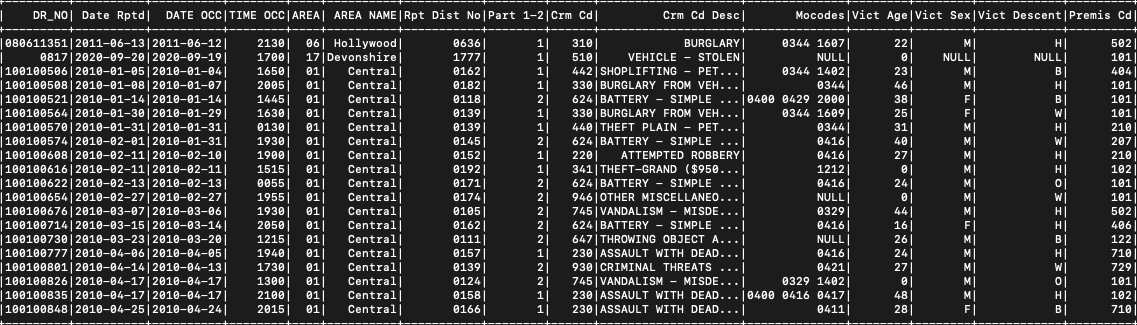
\includegraphics[width=1\linewidth]{df20rowsA.png}
    \caption{\selectlanguage{greek}Πρώτες γραμμές του \selectlanguage{english} Dataframe (1)}
    \label{fig:df20rowsA}
\end{figure}

\begin{figure}[h]
    \centering
    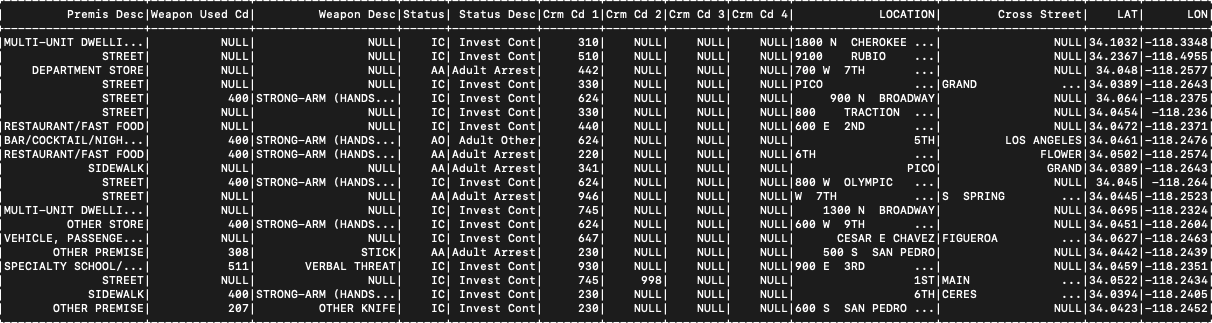
\includegraphics[width=1\linewidth]{df20rowsB.png}
    \caption{\selectlanguage{greek}Πρώτες γραμμές του \selectlanguage{english} Dataframe (2)}
    \label{fig:df20rowsB}
\end{figure}

\selectlanguage{greek} 
\section*{Κύρια Ζητούμενα}
\label{sec:main_z}
Για την υλοποίηση των \selectlanguage{english} Queries \selectlanguage{greek} κληθήκαμε να τα υλοποιήσουμε σε \selectlanguage{english} DataFrame, SQL APIs \selectlanguage{greek} και για το \selectlanguage{english} Query 2 \selectlanguage{greek} και σε \selectlanguage{english} RDD API \selectlanguage{greek} και να συγκρίνουμε τους χρόνους εκτέλεσης για κάθε υλοποίηση.\\
Για κάθε \selectlanguage{english} query \selectlanguage{greek} για να χρονομετρήσουμε την διάρκεια της εκτέλεσης του χρησιμοποιήσαμε την βιβλιοθήκη \selectlanguage{english} \texttt{time} \selectlanguage{greek} της \selectlanguage{english} \texttt{Python} \selectlanguage{greek} και μέσω αυτής προκύπτουν τα αποτελέσματα που παρουσιάζονται στους πίνακες για κάθε ερώτημα. 



\subsection*{Ζητούμενο 3}
\label{subsec:Z3}


Κληθήκαμε να υλοποιήσουμε το \selectlanguage{english} \texttt{Query 1} \selectlanguage{greek} το οποίο ζητά να βρεθούν ανά έτος οι τρεις (3) μήνες με υψηλότερη καταγραφή εγκλημάτων και να παρουσιαστούν τα αποτελέσματα ανά έτος, με φθίνουσα κατάταξη ως προς τον αριθμό των καταγραφών. Για την υλοποίηση δηιουργούμε δύο \selectlanguage{english} derived columns, Year \& Month \selectlanguage{greek} που προκύπτουν από το \selectlanguage{english} DATE OCC, \selectlanguage{greek} μετράμε για κάθε μήνα και χρόνο τις καταγραφές και κρατάμε τους 3 υψηλότερους μήνες. Η εκτέλεση του \selectlanguage{english} Query \selectlanguage{greek} έγινε όπως υποδεικνύεται με 4\selectlanguage{english} Spark executors.\\
\selectlanguage{greek}
\\

Ο Πίνακας 2 παρουσιάζει τα αποτελέσματα του ζητουμένου με την σειρά που αναφέρεται παραπάνω. 
\selectlanguage{english}
\begin{table}[h]
\centering
\begin{tabular}{|c|c|c|c||c|c|c|c|}
\hline
\multicolumn{4}{|c||}{2010-2016} & \multicolumn{4}{c|}{2017-Today} \\ \hline
Year & Month & Crime\_Total & Rank & Year & Month & Crime\_Total & Rank  \\ \hline
2010 & 1     & 11538       & 1    & 2017 & 10    & 20433       & 1    \\ \hline
2010 & 3     & 11513       & 2    & 2017 & 7     & 20193       & 2    \\ \hline
2010 & 4     & 10976       & 3    & 2017 & 1     & 19834       & 3    \\ \hline
2011 & 1     & 18137       & 1    & 2018 & 1     & 6259        & 1    \\ \hline
2011 & 7     & 17283       & 2    & 2018 & 8     & 5815        & 2    \\ \hline
2011 & 10    & 17034       & 3    & 2018 & 7     & 5632        & 3    \\ \hline
2012 & 1     & 17944       & 1    & 2019 & 7     & 19122       & 1    \\ \hline
2012 & 8     & 17661       & 2    & 2019 & 8     & 18979       & 2    \\ \hline
2012 & 5     & 17502       & 3    & 2019 & 3     & 18858       & 3    \\ \hline
2013 & 1     & 8691        & 1    & 2020 & 1     & 5259        & 1    \\ \hline
2013 & 8     & 8008        & 2    & 2020 & 2     & 5132        & 2    \\ \hline
2013 & 12    & 8001        & 3    & 2020 & 5     & 4891        & 3    \\ \hline
2014 & 5     & 5296        & 1    & 2021 & 10    & 19310       & 1    \\ \hline
2014 & 6     & 5248        & 2    & 2021 & 7     & 18663       & 2    \\ \hline
2014 & 7     & 4830        & 3    & 2021 & 8     & 18376       & 3    \\ \hline
2015 & 3     & 10200       & 1    & 2022 & 5     & 20425       & 1    \\ \hline
2015 & 5     & 10018       & 2    & 2022 & 10    & 20280       & 2    \\ \hline
2015 & 7     & 9785        & 3    & 2022 & 6     & 20213       & 3    \\ \hline
2016 & 12    & 15347       & 1    & 2023 & 8     & 19782       & 1    \\ \hline
2016 & 10    & 14995       & 2    & 2023 & 7     & 19718       & 2    \\ \hline
2016 & 1     & 14864       & 3    & 2023 & 1     & 19642       & 3    \\ \hline

\end{tabular}
\caption{Crime Data by Year and Month Descending}
\label{table:crime_data}
\end{table}
\\

\selectlanguage{greek}
Ο Πίνακας 3 παρουσιάζει τους χρόνους μεταξύ των εκτελέσεων στα διαφορετικά \selectlanguage{english} APIs. 
\begin{table}[h]
\centering
\begin{tabular}{|l|l|}
\hline
\textbf{API}    & \textbf{Execution Time (seconds)} \\ \hline
DataDrame       & 11.3895                           \\ \hline
SQL             & 11.4259                           \\ \hline
\end{tabular}
\caption{\selectlanguage{greek} Χρόνοι εκτέλεσης ανά \selectlanguage{english}API - Query 1}
\label{table:execution_times}
\end{table}

\selectlanguage{greek}
Από τους χρόνους δεν φαίνεται ουσιαστική διαφορά στην εκτέλεση. Αυτό οφείλεται ότι για την υλοποίηση και στις δύο πέριπτώσηεις των διαφορετικών \selectlanguage{english} API \selectlanguage{greek} η διαχειρίση των δεδομένων στα πλαίσια των \selectlanguage{english}queries \selectlanguage{greek}είναι βελτιστοποιημένη από το ίδιο το \selectlanguage{english}framework.


\selectlanguage{greek}
\subsection*{Ζητούμενο 4}
\label{subsec:Z4}

Η υλοποίηση του \selectlanguage{english} Query 2 \selectlanguage{greek} έγινε με την χρήση 3 διαφορετικών μεθόδων. Κληθήκαμε να ταξινομήσουμε τα τμήματα της ημέρας, ανάλογα με τις καταγραφές εγκλημάτων που έλαβαν χώρα στο δρόμο και να τα ταξινομήσουμε σε φθίνυσα σειρά των καταγραφών του κάθε τμήματος. Για την υλοποίηση χρησιμοποιήσαμε δική μας συνάρτηση \selectlanguage{english}(UDF - User Defined Function) \selectlanguage{greek} που κατηγοριοποιεί το \selectlanguage{english}
segment \selectlanguage{greek} από τα πρώτα 2 ψηφία του \selectlanguage{english} \texttt{"TIME OCC"} \selectlanguage{greek}. Αρχικά φιλτράρουμε μόνο τα \selectlanguage{english} logs \selectlanguage{greek} που στην στήλη \selectlanguage{english} \texttt{"Premis Desc"} \selectlanguage{greek} έχουν την κατηγορία \selectlanguage{english}"STREET" \selectlanguage{greek}και έπειτα προσθέτουμε νέα στήλη με όνομα \selectlanguage{english}"Day\_Segment" \selectlanguage{greek} της οποίας οι τιμές προκύπτουν από την προαναφερθείσα συνάρτηση. Τέλος, απλά παρουσιάζουμε τα αποτελέσματα ομαδοποιώντας ανά μέρος της ημέρας και κατά φθίνουσα σειρά.\\


Οι χρόνοι για την εκτέλεση του \selectlanguage{english} Query \selectlanguage{greek}στα διαφορετικά \selectlanguage{english}API \selectlanguage{greek}φαίνεται στον Πίνακα 4. Όπως και πριν, έτσι και στο ζητούμνενο αυτό εκτελέστηκε με \selectlanguage{english}4 Spark executors. 

\begin{table}[h]
\centering
\begin{tabular}{|l|r|}
\hline
\textbf{API} & \textbf{Execution Time (seconds)} \\ \hline
DataDrame            & 10.2699                           \\ \hline
SQL           & 8.6825                            \\ \hline
RDD           & 19.3205                          \\ \hline
\end{tabular}
\caption{\selectlanguage{greek} Χρόνοι εκτέλεσης ανά \selectlanguage{english}API - Query 2}
\label{table:query_execution_times}
\end{table}

\selectlanguage{greek}Από τους χρόνους παρατηρούμε μια ελαφρά καλύτερη επίδοση της \selectlanguage{english} SQL \selectlanguage{greek} σε σχέση με το \selectlanguage{english} DataDrame API. \selectlanguage{greek}Αυτό που έχει μεγάλη διαφορά \(x2\) χρόνο είναι το \selectlanguage{english} RDD API \selectlanguage{greek} το οποίο θεωρούμε ότι οφείλεται στο ότι τα άλλα \selectlanguage{english} APIs \selectlanguage{greek} είναι \selectlanguage{english}optimizable \selectlanguage{greek} και το \selectlanguage{english} RDD \selectlanguage{greek} δεν είναι \selectlanguage{english} "schema-aware" \selectlanguage{greek} που το κάνει να είναι λιγότερο αποδοτικό. Τελευταία αιτία που επηρεάζει ως ένα βαθμό τον χρόνο εκτέλεσης του ερωτήματος είναι η μετατροπή του \selectlanguage{english} output \selectlanguage{greek} σε \selectlanguage{english} DataFrame \selectlanguage{greek} για την επίτευξη πιο ευπαρουσίαστης εικόνας αποτελέσματος. \\


Παρακάτω στον Πίνακα 5 φαίνονται τα αποτελέσματα του  \selectlanguage{english} Query 2. 

\begin{table}[h]
\centering
\begin{tabular}{|l|r|}
\hline
Segment   & Count  \\ \hline
Night     & 175928 \\ \hline
Evening   & 136977 \\ \hline
Afternoon & 109270 \\ \hline
Morning   & 91830  \\ \hline
\end{tabular}
\caption{Crimes by Day Segment}
\label{table:segment_count}
\end{table}

\selectlanguage{greek}


\subsection*{Ζητούμενο 5}
\label{subsec:Z5}

Στο Ζητούμενο αυτό \selectlanguage{english}\textbf{(Query 3)} \selectlanguage{greek} σκοπός ήταν για το έτος 2015, να βρούμε τις 3 περιοχές του \selectlanguage{english} Los Angeles \selectlanguage{greek} με υψηλότερο και 3 με χαμηλότερο εισόδημα και έπειτα να βρούμε την καταγωγή των θυμάτων εγκλημάτων και να τα παρουσιάσουμε αθροιστικά, με βάση τον αριθμό καταγραφών για κάθε καταγωγή, σε φθίνουσα σειρά. Η υλοποίηση έγινε ως εξής: 
\begin{itemize}
    \item   Από το κύριο \selectlanguage{english} DataFrame \selectlanguage{greek} κρατάμε μόνο καταγραφές με \selectlanguage{english} "DATE OCC"==2015 \& "Vict Descent"!=Null.\selectlanguage{greek}
    \item   Έπειτα κάνουμε \selectlanguage{english} join \selectlanguage{greek} το τροποποιημένο κύριο \selectlanguage{english} DataFrame \selectlanguage{greek} με το δευτερεύον \selectlanguage{english} Geocoding DataFrame\selectlanguage{greek} στις κοινές συντεταγμένες για να αντιστοιχιστούν τα \selectlanguage{english} "ZIP codes" \selectlanguage{greek} των περιοχών. 
    \item   Από το επόμενο βοηθητικό \selectlanguage{english} DataFrame Income 2015 \selectlanguage{greek} κάνουμε \selectlanguage{english}join \selectlanguage{greek} με το κύριο στην στήλη \selectlanguage{english} "ZIP codes" \selectlanguage{greek} για να αντιστοιχιστεί το εισόδημα. 
    \item   Κρατάμε τα 3 μεγαλύτερα εισοδήματα και \selectlanguage{english} "ZIP codes" \selectlanguage{greek} και αντίστοιχα τα 3 μικρότερα σε μία λίστα. 
    \item   Μέσω βοηθητικής συνάρτησης αποκωδικοποιούμε την καταγωγή σε ολόκληρο όνομα και παρουσιάζουμε την λίστα με τις καταγωγές και τον αριθμό καταγραφών θυμάτων σε φθίνουσα σειρά. 
\end{itemize}

Στον πίνακα 6 παρουσιάζεται το αποτέλεσμα του ζητουμένου. 
\selectlanguage{english}
\begin{table}[h]
\centering
\begin{tabular}{|l|r|}
\hline
\textbf{Vict Descent} & \textbf{Crime Count} \\ \hline
Black                & 914                  \\ \hline
Hispanic             & 859                  \\ \hline
White                & 592                  \\ \hline
Other                & 269                  \\ \hline
Asian                & 84                   \\ \hline
Unknown              & 59                   \\ \hline
Korean               & 8                    \\ \hline
Japanese             & 3                    \\ \hline
Italian              & 2                    \\ \hline
Caucasian            & 2                    \\ \hline
Filipino             & 2                    \\ \hline
\end{tabular}
\caption{Crime Count by Victim Descent in 2015}
\label{table:crime_by_descent}
\end{table}

\selectlanguage{greek}
Για την εκτέλεση κληθήκαμε να συγκρίνουμε τους χρόνους εκτέλεσης για 2, 3 και 4 \selectlanguage{english} Spark executors.\selectlanguage{greek} Τα αποτελέσματα φαίνονται στον πίνακα 7. Οι διαφορές στους χρόνους και η παρατήρηση ότι για λιγότερους \selectlanguage{english} executors \selectlanguage{greek} ο χρόνος είναι καλύτερος έχει ορισμένες πιθανές εξηγήσεις. Αρχικά, το αυτξημένο \selectlanguage{english} overhead \selectlanguage{greek} από διαδικασίες που ανατίθεντα. Έπειτα τα πολλαπλά \selectlanguage{english} joins \selectlanguage{greek} αποδίδουν μη αποδοτικούς χρόνους όταν κατανέμεται το φορτίο, μιας και είναι αποδοτικότερο κάποια από αυτά να γίνουν σειριακά.
\selectlanguage{english}
\begin{table}[h]
\centering
\begin{tabular}{|l|r|r|r|}
\hline
API / \# of executors & 4             & 3             & 2             \\ \hline
DataFrame            & 20.9337 sec & 21.7335 sec & 16.3127 sec \\ \hline
SQL           & 18.4258 sec & 16.4078 sec & 12.4836 sec \\ \hline
\end{tabular}
\caption{\selectlanguage{greek} Χρόνοι εκτέλεσης για διαφορετικό αριθμό\selectlanguage{english} executors per API - Query 3}
\label{table:query3_execution_different_executors}
\end{table}


\selectlanguage{greek}


\subsection*{Ζητούμενο 6}
\label{subsec:Z6}

Όσον αφορά το ζητούμενο αυτό μας ανατέθηκε το τελευταίο και πιο εκτενές σε περιπτώσεις \selectlanguage{english} \textbf{Query (4)}. \selectlanguage{greek}Για τον υπολογισμό των αποστάσεων χρησιμοποιήσαμε διαφορετικη υλοποίση συνάρτησης από την προτεινόμενη. Επίσης, για την αποφυγή λάθος αποτελεσμάτων και μεγαλύτερων χρόνων εκτέλεσης, αφαιρέσαμε τα \selectlanguage{english} logs \selectlanguage{greek} με συντεταγμένες που ανήκουν στο \selectlanguage{english} Null Island\footnote{Null Island faulty LAT,LON:\selectlanguage{greek}Ένα σημαντικό μέρος των συντεταγμένων των καταγραφών φέρεται να έχει περασμένες τις "μηδενικές συντεταγμένες", και προκύπτουν αποτελέσματα χωρίς λογική συνέχεια.}.\\
\selectlanguage{english}
\begin{table}[h]
\centering
\begin{tabular}{|c|c|c|}
\hline
Year & Average Distance in km & Count \\ \hline
2010 & 2.651 & 5486 \\ \hline
2011 & 2.793 & 7232 \\ \hline
2012 & 2.836 & 6532 \\ \hline
2013 & 2.731 & 2271 \\ \hline
2014 & 2.683 & 2320 \\ \hline
2015 & 2.654 & 3500 \\ \hline
2016 & 2.734 & 6076 \\ \hline
2017 & 2.724 & 7786 \\ \hline
2018 & 2.566 & 2242 \\ \hline
2019 & 2.74  & 7129 \\ \hline
2020 & 2.49  & 2248 \\ \hline
2021 & 2.64  & 9745 \\ \hline
2022 & 2.609 & 10026 \\ \hline
2023 & 2.556 & 9017 \\ \hline
\end{tabular}
\caption{Average Distance and Count by Year - A}
\label{table:average_distance_counta}
\end{table}
\clearpage
\selectlanguage{greek}
Το πρώτο μέρος του \selectlanguage{english} Query \selectlanguage{greek} και το α' ζητούμενο αφορά τον υπολογισμό εγκλημάτων στα οποία καταγράφηκε χρήση (οποιασδήποτε μορφής) πυροβόλου όπλου και η μέση απόσταση από το αστυνομικό τμήμα που ανέλαβε το περιστατικό.Στον πίνακα 8 φαίνονται τα αποτελέσματα του ζητουμένου. Υλοποιήθηκε με την βοήθεια του δευτερεύοντος \selectlanguage{english} DataFrame: LAPD police stations \selectlanguage{greek} στα εξής βήματα:
\begin{itemize}
    \item   Φιλτράρω των κωδικό των πυροβόλων όπλων "$1xx$" από την στήλη του κύριου \selectlanguage{english}DataFrame, "Weapon Used Cd".\selectlanguage{greek}
    \item   Κάνω \selectlanguage{english} join \selectlanguage{greek} τα δύο \selectlanguage{english} DataFrames (main - LAPD) \selectlanguage{greek} στο κοινό πεδίο τους \selectlanguage{english} \texttt{"main.AREA==lapd.PREC"}.
    \item   \selectlanguage{greek}Υπολογίζω την απόσταση σε νέα στήλη και τέλος ανα χρόνο κάνω \selectlanguage{english} sort \selectlanguage{greek} για κάθε χρονιά τις καταγραφές.
\end{itemize}

\selectlanguage{english}
\begin{table}[h]
\centering
\begin{tabular}{|l|c|r|}
\hline
Division        & Average Distance in km & Count \\ \hline
SOUTHWEST       & 2.606 & 71344 \\ \hline
77TH STREET     & 2.644 & 67523 \\ \hline
CENTRAL         & 1.006 & 63052 \\ \hline
RAMPART         & 1.531 & 55229 \\ \hline
SOUTHEAST       & 2.087 & 45910 \\ \hline
HOLLYWOOD       & 1.428 & 44560 \\ \hline
NEWTON          & 2.047 & 39366 \\ \hline
HOLLENBECK      & 2.592 & 38609 \\ \hline
HARBOR          & 3.939 & 38016 \\ \hline
OLYMPIC         & 1.749 & 30840 \\ \hline
NORTHEAST       & 3.980 & 27356 \\ \hline
WILSHIRE        & 2.412 & 26850 \\ \hline
MISSION         & 4.710 & 26797 \\ \hline
PACIFIC         & 3.895 & 25889 \\ \hline
VAN NUYS        & 2.138 & 25045 \\ \hline
WEST VALLEY     & 3.375 & 24598 \\ \hline
NORTH HOLLYWOOD & 2.536 & 23426 \\ \hline
TOPANGA         & 3.512 & 19910 \\ \hline
FOOTHILL        & 4.240 & 19710 \\ \hline
WEST LOS ANGELES& 3.648 & 19154 \\ \hline
DEVONSHIRE      & 3.987 & 18250 \\ \hline
\end{tabular}
\caption{Average Distance and Count by Division - A}
\label{table:division_distance_count_a}
\end{table}




\selectlanguage{greek}
Στο β' ζητούμενο του μέρους καλούμαστε να υπολογίσουμε τις καταγραφές εγκλημάτων με χρήση όπλου (οποιοσδήποτε κωδικός δίαφορος του \selectlanguage{english}Null)\selectlanguage{greek} και να τα παρουσιάσουμε ανά Αστυνομικό Τμήμα, στα οποία ανατέθηκαν τα συμβάντα. Το αποτέλεσμα φαίνεται στον πίνακα 9. 

\clearpage
Τα βήματα της υλοποίσης:
\begin{itemize}
    \item   Φιλτράρισμα των \selectlanguage{english} non-Null \selectlanguage{greek} τιμών του πεδίου \selectlanguage{english} "Weapon Used Cd".
    \item   Join Main \& LAPD DataFrame \selectlanguage{greek} ώστε \selectlanguage{english} \texttt{"main.AREA==lapd.PREC"}.
    \item   \selectlanguage{greek}Υπολογισμός απόστασης και παρουσίαση καταγραφών ανά Αστυνομικό τμήμα.
\end{itemize}


\selectlanguage{english}
\begin{table}[ht]
\centering
\begin{tabular}{|c|c|r|}
\hline
Year & Average Distance in km & Count \\ \hline
2010 & 2.28   & 5486  \\ \hline
2011 & 2.462  & 7232  \\ \hline
2012 & 2.506  & 6532  \\ \hline
2013 & 2.416  & 2271  \\ \hline
2014 & 2.16   & 2320  \\ \hline
2015 & 2.462  & 3500  \\ \hline
2016 & 2.415  & 6076  \\ \hline
2017 & 2.392  & 7786  \\ \hline
2018 & 2.35   & 2242  \\ \hline
2019 & 2.43   & 7129  \\ \hline
2020 & 2.269  & 2248  \\ \hline
2021 & 2.353  & 9745  \\ \hline
2022 & 2.313  & 10026 \\ \hline
2023 & 2.275  & 9017  \\ \hline
\end{tabular}
\caption{Average Distance and Count by Year - B}
\label{table:year_distance_count_b}
\end{table}





\clearpage
\selectlanguage{greek}
Στο δεύτερο μέρος κληθήκαμε να υλοποιήσουμε τα ίδια ερωτήματα αλλά με την \textbf{διαφορά} ότι τα αστυνομικά τμήματα που θα λαμβάναμε στο τέλος για τον υπολογισμό της απόστασης θα ήταν αυτά που έχουν την \textbf{μικρότερη απόσταση από τον τόπο της καταγραφής} και όχι το τμήμα που ανέλαβε την υπόθεση.

\selectlanguage{english}
\begin{table}[ht]
\centering
\begin{tabular}{|l|c|r|}
\hline
Division        & Average Distance in km & Count \\ \hline
SOUTHWEST       & 2.084 & 67692 \\ \hline
HOLLYWOOD       & 1.863 & 59232 \\ \hline
CENTRAL         & 0.852 & 57332 \\ \hline
RAMPART         & 1.331 & 54937 \\ \hline
77TH STREET     & 1.672 & 54643 \\ \hline
WILSHIRE        & 2.516 & 46857 \\ \hline
OLYMPIC         & 1.691 & 44018 \\ \hline
SOUTHEAST       & 2.281 & 42670 \\ \hline
HOLLENBECK      & 2.576 & 39151 \\ \hline
VAN NUYS        & 2.796 & 37856 \\ \hline
HARBOR          & 3.683 & 36912 \\ \hline
NEWTON          & 1.613 & 29835 \\ \hline
PACIFIC         & 3.869 & 24523 \\ \hline
WEST VALLEY     & 2.811 & 24501 \\ \hline
NORTH HOLLYWOOD & 2.602 & 24077 \\ \hline
FOOTHILL        & 3.977 & 23845 \\ \hline
TOPANGA         & 3.053 & 20287 \\ \hline
NORTHEAST       & 3.757 & 20214 \\ \hline
MISSION         & 3.787 & 17693 \\ \hline
WEST LOS ANGELES& 2.697 & 15700 \\ \hline
DEVONSHIRE      & 2.844 & 9459  \\ \hline
\end{tabular}
\caption{Average Distance and Count by Division - B}
\label{table:division_distance_count_b}
\end{table}






\selectlanguage{greek}
Στο α' ζητούμενο η υλοποίηση είναι παρόμοια με την υλοποίηση α' του πρώτου μέρους. Για να βρούμε όμως το πλησιέστερο Αστυνομικό Τμήμα χρησιμοποιούμε \selectlanguage{english}\texttt{cross join} \selectlanguage{greek} το οποίο είναι πολύ πιο κοστοβόρο και χρονοβόρο, αλλά είναι ο πιο απλός τρόπος για να βρρεθεί η ελάχιστη απόσταση μεταξύ κάθε καταγραφής εγκλήματος και αστυνομικού τμήματος. Από τις αποστάσεις κρατάμε το \selectlanguage{english}log \selectlanguage{greek} με την ελάχιστη τιμή και συνεχίζουμε την παρουσίαση του ζητήματος όπως και στο πρώτο μέρος. Αντίστοιχα πράττουμε και στο β' ερώτημα του δευτέρου μέρους με χρήση \selectlanguage{english} cross join \selectlanguage{greek} και η υπόλοιπη διαδικασία παραμένει ίδια.Τα αποτελέσματα του δεύτερου μέρους για το α' και β' ερώτημα, παρουσιάζονται στους πίνακες 10 και 11 αντίστοιχα.\\






\clearpage
\selectlanguage{english}
\begin{table}[ht]
\centering
\begin{tabular}{|l|r|}
\hline
\textbf{Query}      & \textbf{Execution Time (seconds)} \\ \hline
DF\_1a        & 12.7367                           \\ \hline
SQL\_1a       & 11.2110                           \\ \hline
DF\_1b        & 13.2750                           \\ \hline
SQL\_1b       & 14.4775                           \\ \hline
DF\_2a        & 25.0340                           \\ \hline
SQL\_2a       & 17.1889                           \\ \hline
DF\_2b        & 61.8993                           \\ \hline
SQL\_2b       & 63.0198                           \\ \hline
\end{tabular}
\caption{\selectlanguage{greek}Χρόνοι εκτέλεσης για τις περιπώσεις του \selectlanguage{english} Query 4}
\label{table:query4_execution_times}
\end{table}



\selectlanguage{greek}
Οι συγκρίσεις μεταξύ των χρόνων εκτέλεσης των \selectlanguage{english}Queries \selectlanguage{greek} και των παραλλαγών τους στα διαφορετικά \selectlanguage{english}APIs (4 executors) \selectlanguage{greek}φαίνονται στον πίνακα 12. Για τα ερωτήματα του πρώτου μέρους παρατηρούμε παρόμοιους χρόνους για τα δύο \selectlanguage{english} APIs \selectlanguage{greek}, ενώ για το δεύτερο μέρος το α' ερώτημα μπορούμε να δούμε ότι υπάρχει μια υπεροχή της \selectlanguage{english} SQL \selectlanguage{greek}όσον αφορά το \selectlanguage{english} efficiency \selectlanguage{greek}που χειρίζεται το \selectlanguage{english} cross join \selectlanguage{greek} και αποδίδει μικρότερο χρόνο. Για το τελευταίο ερώτημα είναι σαφής η μεγάλη διαφορά στον χρόνο εκτέλεσης σε σχέση με τα υπόλοια (και για τα δύο \selectlanguage{english} APIs) \selectlanguage{greek} αφού χειρίζεται \selectlanguage{english} cross join \selectlanguage{greek}και υπολογισμό τιμή για πολύ μεγαλύτερο όγκο δεδομένων. 


\selectlanguage{greek}
\subsection*{Ζητούμενο 7}
\label{subsec:Z7}


Στο τελικό ζητούμενο ζητήθηκε για τα \selectlanguage{english} "joins" \selectlanguage{greek} των \selectlanguage{english} \texttt{Query 3 \& 4},
\selectlanguage{greek} να χρησιμοποιηθούν οι μέθοδοι \selectlanguage{english}\texttt{hint() \& explain()} \selectlanguage{greek} των \selectlanguage{english} DataFrame/SQL APIs \selectlanguage{greek}ώστε να εκτελεστούν με διαφορετικό τρόπο και να πάρουμε πλάνο μέσω του \selectlanguage{english} Spark History UI \selectlanguage{greek} για τις αποδοτικότερες στρατηγικές \selectlanguage{english} join.\\ 






\selectlanguage{greek}Παρακάτω παρουσιάζονται στον Πίνακα 13 ενδεικτικά δεδομένα από το \selectlanguage{english} Spark History UI \selectlanguage{greek}. Εκεί τρέχουμε τις εντολές \selectlanguage{english}\texttt{hint() \& explain()} \selectlanguage{greek} για να δούμε την απόδοση του κάθε \selectlanguage{english} query \selectlanguage{greek} όσον αφορά τον χρόνο εκτέλεσης, της κατανομής δεδομένων και του \selectlanguage{english} shuffle \selectlanguage{greek} μεταξύ των \selectlanguage{english} workers.\\
\selectlanguage{greek}
Οι εντολές χρησιμοποιούνται ως εξής: 
\begin{itemize}
    \item   Στο \selectlanguage{english} \texttt{join: df\_joined = df1.join(df2.hint("JOIN TYPE"), "condition")}
    \item   Join types: \texttt{broadcast, merge, shuffle\_hash, shuffle\_hash\_nl}
    
    \item   \selectlanguage{greek}Για την παρουσίαση του πλάνου (\selectlanguage{english}join strategy): \texttt{df\_joined.explain()}
\end{itemize}


% ## use df.hint("JOIN TYPE") join types: broadcast, merge, shuffle_hash, shuffle_hash_nl  for the right plan




\selectlanguage{english}
\begin{table}[ht]
\centering
\caption{Spark History UI - Join Types Comparison}
\label{table:join_comparison}
\begin{tabular}{|l|c|c|c|}
\hline
\textbf{Join Type} & \textbf{Ex. Time} & \textbf{Data Shuffle} & \textbf{CPU Usage/load} \\
\hline
\textbf{Broadcast} & 35s & \foreignlanguage{greek}{Μικρό} data shuffle & \foreignlanguage{greek}{Όμοια κατ.} \\
\hline
\textbf{Merge} & 38s & \foreignlanguage{greek}{Μεγάλο} data shuffle & \foreignlanguage{greek}{Σχ. όμοια καταν} \\
\hline
\textbf{Shuffle\_hash} & 35s & \foreignlanguage{greek}{Μεγάλο} data shuffle & \foreignlanguage{greek}{Σχ. ανόμοια κατ.} \\
\hline
\textbf{shuffle\_replicate\_nl} & >1m & \foreignlanguage{greek}{Πολύ Μεγάλο} shuffle & \foreignlanguage{greek}{Πολύ ανόμοια κατ.} \\
\hline
\end{tabular}
\end{table}

\selectlanguage{greek}
Από τα δεδομένα και το \selectlanguage{english}text plan \selectlanguage{greek}που πήραμε για τα \selectlanguage{english}queries \selectlanguage{greek}μέσω της εντολής \selectlanguage{english}\texttt{.explain()}\selectlanguage{greek} (χρησιμποιείται ως) στο μέρος του \selectlanguage{english}join \selectlanguage{greek}που χρησιμοποιούμε, εξάγουμε τα παρακάτω συμπεράσματα: 
\begin{itemize}
    \item   Για τα απλά \selectlanguage{english}joins \selectlanguage{greek}παρατηρούμε ότι η πιο αποδοτική στρατηγική είναι το \selectlanguage{english} "broadcast". \selectlanguage{greek}Για μεγάλα \selectlanguage{english} DataFrames \selectlanguage{greek} η επίδοση μειώνεται καθώς δεν μπορεί να κατανεμηθεί όμοια το φορτίο στους \selectlanguage{english} executors \selectlanguage{greek} και πολλές εκτελέσεις τείνουν να "κολλανε" σε έναν \selectlanguage{english} worker \selectlanguage{greek} με τους υπόλοιπους να περιμένουν απάντηση από αυτόν. 

    \item   Όσον αφορά την χρήση \selectlanguage{english} "cross-join" \selectlanguage{greek} μπορούμε να συμπεράνουμε ότι είναι μία αρκετά κοστοβόρα διαδικασία και δεν συνίσταται για συνδυασμούς μεγάλων όγκων δεδομένων. Στην περίπτωση που χρησιμοποιήθηκε τα δεδομένα έχουν ήδη φιλτραριστεί και έχουν περιορισθεί σε $100-300$ χιλιάδες γραμμές το πολύ. Παρόλα αυτά η χρήση του \selectlanguage{english} broadcast join \selectlanguage{greek} φαίνεται να είναι η πιο αποδοτική σε κάθε περίπτωση, που θέλουμε να αντλήσουμε πληροφορίες απο μικρότερο \selectlanguage{english} DataFrame. 
\end{itemize}




\selectlanguage{greek}
\section*{Παράρτημα}
\label{sec:appendix}
\subsection*{Παράρτημα Α - Kώδικας Boηθητικών συναρτήσεων}
\label{subsec:apend_A}
Στο παράρτημα αυτό παρατίθεται κώδικας και επεξήγηση του σε σημεία που θεωρούμε οτι χρήζουν περαιτέρω ανάλυσης. 
\selectlanguage{english}
\begin{lstlisting}[language=Python,caption={UDF registration script}]
from pyspark.sql.functions import udf
from pyspark.sql.types import StringType, FloatType
from math import radians, sin, cos, sqrt, atan2

descent_mapping = {
    'A': 'Asian', 'B': 'Black', 'C': 'Caucasian', 'D': 'Indian',
    'F': 'Filipino', 'G': 'German', 'H': 'Hispanic', 'I': 'Italian',
    'J': 'Japanese', 'K': 'Korean', 'L': 'Laotian', 'O': 'Other',
    'P': 'Pacific Islander', 'S': 'Samoan', 'U': 'Hawaiian',
    'V': 'Vietnamese', 'W': 'White', 'X': 'Unknown',
    'Z': 'Asian Indian', '-': 'Not Specified', None: 'Unknown'
}

def map_descent(code):
    return descent_mapping.get(code, 'Unknown')

def get_distance(lat1, lon1, lat2, lon2):
    lat1, lon1, lat2, lon2 = map(radians, [float(lat1), float(lon1), float(lat2), float(lon2)])
    dlat = lat2 - lat1
    dlon = lon2 - lon1
    a = sin(dlat / 2)**2 + cos(lat1) * cos(lat2) * sin(dlon / 2)**2
    c = 2 * atan2(sqrt(a), sqrt(1 - a))
    radius = 6371.0
    return radius * c

def get_day_segment(time_str):
    try:
        hour = int(time_str['TIME OCC'][:2])

        # Classify into day segments
        if 5 <= hour < 12:
            return 'Morning'
        elif 12 <= hour < 17:
            return 'Afternoon'
        elif 17 <= hour < 21:
            return 'Evening'
        else:
            return 'Night'
    except ValueError:
        return 'Unknown'

# Registering UDFs
map_descent_udf = udf(map_descent, StringType())
get_distance_udf = udf(get_distance, FloatType())
get_day_segment_udf = udf(get_day_segment, StringType())
\end{lstlisting}
\selectlanguage{greek}
Όσον αφορά το \selectlanguage{english}\texttt{udfs.py} script \selectlanguage{greek}που φαίνεται στο παραπάνω απόκομμα 1, παρουσιάζονται συγκεντρωτικά οι \selectlanguage{english}\texttt{User Defined Function} \selectlanguage{greek} που χρησιμοποιήσαμε και κάναμε \selectlanguage{english} regsiter \selectlanguage{greek} στο σύστημα για τον υπολογισμό των αποστάσεων (Ζητούμενο 6~\ref{subsec:Z6}), ο διαχωρισμός του μέρους της μέρας (Ζητούμενο 4~\ref{subsec:Z4}) και η αντιστοίχηση του χαρακτήρα προέλευσης με το κανονικό όνομα (Ζητούμενο 5~\ref{subsec:Z5}).


Σεγκεκριμένα για την συνάρτηση υπολογισμού της απόστασης \selectlanguage{english} \texttt{get\_distance} \selectlanguage{greek} χρησιμοποίησαμε διαφορετική υλοποίηση από την προτεινόμενη (\selectlanguage{english} geopy library). \selectlanguage{greek}Μετατρέπουμε τις συντεταγμένες σε \selectlanguage{english} radians \selectlanguage{greek},υπολογίζουμε τις διαφορές των συντεταγμένων και χρησιμοποιούμε τον τύπο \selectlanguage{english} haversine \selectlanguage{greek} για τον υπολογισμό της γωνιακής απόστασης \selectlanguage{english}\textbf{c}\selectlanguage{greek} που πολλαπλασιαζουμε με την ακτίνα της Γης σε χιλιόμετρα.


\subsection*{Παράρτημα B - Kώδικας Ερωτημάτων}
\label{subsec:apend_B}
\selectlanguage{english}
\begin{lstlisting}[language=Python, caption={Query 3 - SQL}]
spark.sql("""
    -- Filter for 2015 crimes and select required columns
    WITH Crimes2015 AS (
        SELECT DR_NO, `DATE OCC`, `AREA NAME`, `Vict Descent`, LOCATION, LAT, LON
        FROM df_main
        WHERE YEAR(`DATE OCC`) = 2015 AND `Vict Descent` IS NOT NULL
    ),
    -- Join with geodf to get ZIP codes
    CrimeWithZip AS (
        SELECT c.*, g.ZIPcode
        FROM Crimes2015 c
        INNER JOIN geodf g ON c.LAT = g.LAT AND c.LON = g.LON
    ),
    -- Join with income data
    CrimeWithIncome AS (
    SELECT cwz.*, i.`Zip Code`, 
           CAST(REGEXP_REPLACE(i.`Estimated Median Income`, '[\\$,]', '') AS DOUBLE) AS IncomeNumeric
    FROM CrimeWithZip cwz
    INNER JOIN incdf15 i ON cwz.ZIPcode = i.`Zip Code`
    ),
    -- Get distinct ZIP codes based on income
    DistinctZipIncome AS (
        SELECT DISTINCT `Zip Code`, IncomeNumeric
        FROM CrimeWithIncome
    ),
    -- Get top 3 and bottom 3 ZIP codes
    TopBottomZip AS (
        (SELECT `Zip Code` FROM DistinctZipIncome ORDER BY IncomeNumeric DESC LIMIT 3)
        UNION ALL
        (SELECT `Zip Code` FROM DistinctZipIncome ORDER BY IncomeNumeric ASC LIMIT 3)
    ),
    -- Filter crimes for these ZIP codes
    FilteredCrimes AS (
        SELECT *
        FROM CrimeWithIncome
        WHERE `Zip Code` IN (SELECT `Zip Code` FROM TopBottomZip)
    )
    SELECT 
        COALESCE(
    CASE `Vict Descent`
        WHEN 'A' THEN 'Asian'
        WHEN 'B' THEN 'Black'
        WHEN 'C' THEN 'Caucasian'
        WHEN 'D' THEN 'Indian'
        WHEN 'F' THEN 'Filipino'
        WHEN 'G' THEN 'German'
        WHEN 'H' THEN 'Hispanic'
        WHEN 'I' THEN 'Italian'
        WHEN 'J' THEN 'Japanese'
        WHEN 'K' THEN 'Korean'
        WHEN 'L' THEN 'Laotian'
        WHEN 'O' THEN 'Other'
        WHEN 'P' THEN 'Pacific Islander'
        WHEN 'S' THEN 'Samoan'
        WHEN 'U' THEN 'Hawaiian'
        WHEN 'V' THEN 'Vietnamese'
        WHEN 'W' THEN 'White'
        WHEN 'X' THEN 'Unknown'
        WHEN 'Z' THEN 'Asian Indian'
        WHEN '-' THEN 'Not Specified'
        ELSE 'Unknown'
    END,
    'Unknown'
) AS `Vict Descent Name`,
        COUNT(*) AS `Crime Count`
    FROM FilteredCrimes
    GROUP BY `Vict Descent Name`
    ORDER BY `Crime Count` DESC
""").show()    
\end{lstlisting}


\selectlanguage{greek}
Για το απόκομμα 2 που περιλαμβάνει την υλοποίηση του \selectlanguage{english}Query 3 (SQL)~\ref{subsec:Z5} \selectlanguage{greek}παρατίθεται η επεξήση σε βήματα: 
\begin{itemize}
    \item   Αρχικά φιλτράρουμε τις καταγραφές μόνο από το 2015 με έγκυρες συντεταγμένες
    \item   Από αυτό κάνουμε \selectlanguage{english} join \selectlanguage{greek} με τις συντεταγμένες του \selectlanguage{english}geocoding \selectlanguage{greek} για να κρατήσουμε το \selectlanguage{english} Zip Code. 
    \item   \selectlanguage{greek} Κάνουμε \selectlanguage{english} join \selectlanguage{greek} με το \selectlanguage{english} Income 2015 \selectlanguage{greek} στο \selectlanguage{english} ZIP Code \selectlanguage{greek} και μετατρέπουμε την στήλη \selectlanguage{english} 'Estimated Median Income' \selectlanguage{greek} σε αριθμό χωρίς το μέρος του νομίσματος.
    \item   Κρατάμε μόνο \selectlanguage{english} distinct Zip codes \selectlanguage{greek} για να πάρουμε τα σωστά αποτελέσματα ανάλογα με το εισόδημα.
    \item   Επιλέγουμε τα 3 μικρότερα και 3 μεγαλύτερα εισοδήματα.
    \item   Στο \selectlanguage{english} Temporary View 'FilteredCrime' \selectlanguage{greek} κρατάμε καταγραφές με \selectlanguage{english} Zip Code \selectlanguage{greek} που ταιριάζει με τα επιλεγμένα 6. 
    \item   Στο τέλος κάνουμε μετάφραση των ονομάτων και μετράμε τις καταγραφές για κάθε περίπτωση, κάνουμε \selectlanguage{english} Group By \selectlanguage{greek}βάσει της καταγωγής και τα παρουσιάζουμε σε φθίνουσα σειρά. 
\end{itemize}

\selectlanguage{english}
\begin{lstlisting}[language=Python, caption={Query 4 2a - SQL}]
spark.sql("""
    WITH FilteredData AS (
        SELECT
            DR_NO, LAT, LON, `DATE OCC`, AREA
        FROM df_main
        WHERE CAST(`Weapon Used Cd` / 100 AS INT) = 1
    ),
    CrossJoined AS (
        SELECT
            f.DR_NO, f.LAT, f.LON, f.`DATE OCC`, f.AREA,
            l.Y, l.X, l.DIVISION
        FROM FilteredData f
        CROSS JOIN lapd l
    ),
    Distances AS (
        SELECT
            *,
            get_distance(LAT, LON, Y, X) AS DISTANCE,
            ROW_NUMBER() OVER (PARTITION BY DR_NO ORDER BY get_distance(LAT, LON, Y, X)) AS rank
        FROM CrossJoined
    ),
    ClosestPrecincts AS (
        SELECT
            DR_NO, `DATE OCC`, AREA, DIVISION, DISTANCE
        FROM Distances
        WHERE rank = 1
    )
    SELECT
        YEAR(`DATE OCC`) AS Year,
        ROUND(MEAN(DISTANCE), 3) AS `average distance in km`,
        COUNT(*) AS Count
    FROM ClosestPrecincts
    GROUP BY YEAR(`DATE OCC`)
    ORDER BY YEAR(`DATE OCC`)
""").show()
    
\end{lstlisting}

\selectlanguage{greek} 
Το απόκομμα 3 αποτελεί την υλοποίηση του ερωτήματος α' του δεύτερου μέρους όσον αφορά το \selectlanguage{english}Query 4~\ref{subsec:Z6}. \selectlanguage{greek} Θεωρούμε την υλοποίηση άξια αναφοράς καθώς χρησιμοποιούμε το \selectlanguage{english} "cross join". \selectlanguage{greek}Παρακάτω τα βήματα:
\selectlanguage{greek}
\begin{itemize}
    \item   Αρχικά φιλτράρουμε από το \selectlanguage{english} DataFrame\selectlanguage{greek} μόνο τις χρήσιμες στήλες, καθώς οι μετατροπές που θα κάνουμε παρακάτω θα είναι κοστοβόρες και χρονοβόρες, και κρατάμε μόνο τις καταγραφές με κωδικό όπλου που αρχίζει με $1$.
    \item   Στη συνέχεια εκτελούμε \selectlanguage{english} cross join \selectlanguage{greek} των καταγραφών που έχουμε με τις γεωγραφιές συντεταγμένες του \selectlanguage{english} DataFrame LAPD. 
    \item   \selectlanguage{greek}Στο επόμενο βήμα χρησιμοποιούμε την δική μας συνάρτηση \selectlanguage{english}\texttt{get\_distance} \selectlanguage{greek} για τον υπολογισμό κάθε απόστασης.
    \item   Με το \selectlanguage{english}\texttt{ROW\_NUMBER()} \selectlanguage{greek} αποδίδουμε ένα \selectlanguage{english}"rank" \selectlanguage{greek}για κάθε τμήμα και κάθε για κάθε έγκλημα σορταρισμένο βάσει της απόστασης. Έτσι βρίσκουμε το πλησιέστερο Α.Τ. στο έγκλημα. 
    \item   Από αυτά κρατάμε μόνο όσες καταγραφές έχουν \selectlanguage{english}"Rank==1"\selectlanguage{greek}, δηλαδή είναι οι καταγραφές με την απόσταση του πλησιέστερου τμήματος.
    \item   Τέλος, παρουσιάζω τα εγκλήματα ανά έτος και τον αριθμό των καταγραφών, έχοντας βρει την μέση απόσταση για κάθε έγκλημα της συγκεκτριμένης χρονιάς. 
\end{itemize}

\selectlanguage{english}
\begin{lstlisting}[language=Python, caption={Query 4 2a - DF}]
    df_main = df_main.filter((col("LAT") != 0.0) & (col("LON") != 0.0))
# Select relevant columns and perform a cross join
df_main_firearms = df_main.filter((col("Weapon Used Cd") / 100).cast("int") == 1).select("DR_NO", "LAT", "LON", "DATE OCC", "AREA")
cross_joined = df_main_firearms.crossJoin(lapd)

with_distances = cross_joined.withColumn("DISTANCE", get_distance(col("LAT"), col("LON"), col("Y"), col("X")))

windowSpec = Window.partitionBy(cross_joined["DR_NO"]).orderBy("DISTANCE")

ranked = with_distances.withColumn("rank", row_number().over(windowSpec))

# Filter to keep only the closest precinct (rank = 1) for each row in the main DataFrame
closest_precincts = ranked.filter(col("rank") == 1).drop("rank")

# Now, closest_precincts DataFrame has each row from df_main along with the details of its closest precinct
q4_2a = closest_precincts.groupBy(year(closest_precincts["DATE OCC"]).alias("Year")) \
    .agg(round(avg("DISTANCE"), 3).alias("average distance in km"), count("*").alias("Count")) \
    .orderBy("Year", ascending=True)

q4_2a.show(q4_2a.count())
\end{lstlisting}


\selectlanguage{greek}
Για το τελευταίο απόκκομα (4), που είναι υλοποίηση σε \selectlanguage{english} Python - Spark DataFrame API,\selectlanguage{greek} σχολιάζουμε τις ουσιαστικές αλλαγές σε σχέση με την προηγούμενη υλοποίηση σε \selectlanguage{english} SQL API. \selectlanguage{greek}Στο κομμάτι αυτό, συνεπώς, θα σχολιάσουμε το φιλτράρισμα των κοντινότερων αποστάσεων. 


Μετά το \selectlanguage{english} cross join \selectlanguage{greek} χρησιμποιούμε το \selectlanguage{english}\texttt{Window.partitionBy()} \selectlanguage{greek} που χωρίζει το \selectlanguage{english} DataFrame view \selectlanguage{greek} στο οποίο εγραζόμαστε, σε ομάδες ανάλογα με το \selectlanguage{english} unique log identifier "DR\_NO" \selectlanguage{greek} που αντιστοιχεί σε κάθε καταγεγραμμένο έγκλημα. Έπειτα, προσθέτουμε την στήλη \selectlanguage{english}"rank" \selectlanguage{greek} και όπως πριν κρατάμε τις καταγραφές με "βαθμό" ίσο με ένα, δηλαδή την μικρότερη απόσταση. Τέλος, ομαδοποιούμε και παρουσιάζουμε όπως και στην προηγούμενη υλοποίηση. 


Για τις υπόλοιπες υλοποιήσεις δεν παρατίθεται κώδικας ή αποκόμματα εντός της αναφοράς, καθώς την καθιστά υπερβολικά εκτενή. Περιγράψαμε αυτές που θεωρήσαμε ότι ήταν σημαντικότερες ή άξιες αναφοράς. Για αναλυτικότερη περιήγηση στις υλοποιήσεις, ο κώδικας υπάρχει στο \selectlanguage{english}Github repository\footnote{https://github.com/georgebaris/advanced\_db\_project}.

\end{document}

